\section{Parte B}

    \begin{tabular} { |p{2.2cm}|p{3.6cm}|p{3.6cm}|p{3.4cm}|p{2.25cm}|  }
        \hline
       
        \textbf{Comando} & \textbf{Protocolo de Aplicação} & \textbf{Protocolo de Transporte} & \textbf{Porta de Atendimento} & \textbf{Overhead} \\
        
        \hline
        \textbf{Ping} & Não aplicável & Não aplicável & Não aplicável & Não aplicável \\
        
        \hline
        \textbf{Traceroute} & DNS & TCP e UDP & 33434-33494  & $\simeq$ 16.09\% \\

        \hline
        \textbf{FTP} & FTP & TCP & 21 (dados: 20) & $\simeq $ 38.14\% \\

        \hline
        \textbf{TFTP} & TFTP & UDP & 69 & $\simeq$ 3.34\% \\

        \hline
        \textbf{ssh} & SSH & TCP & 22 & $\simeq$ 11.22\% \\

        \hline
        \textbf{telnet} & TELNET & TCP & 23 & $\simeq$ 20.62\% \\

        \hline
        \textbf{browser} & HTTP & TCP & 80 & $\simeq$ 2.48\% \\

        \hline
        \textbf{nslookup} & DNS & UDP & 53 & $\simeq$ 12.69\%  \\

        \hline
        \textbf{BitTorrent} & HTTP & TCP & 6881-6889 & $\simeq$ 15.68\% \\

        \hline
        \textbf{XMPP} & HTTP & TCP & 5222 & $\simeq$ 21.14\% \\

        \hline
        \textbf{Git} & HTTP, HTTPS ou SSH & TCP & 9418 & $\simeq$ 24.63\% \\
        
        \hline
    \end{tabular}

    \vspace{15pt}
    \textbf{\large Ping}

    Como resulta  simplesmente da utilização de pacotes ICMP, podemos concluir de imediato que não é aplicado qualquer protocolo de transporte a partir do momento em que o comando é executado, como tal não é possível preencher a células apresentadas.

    \begin{figure}
        \centering
        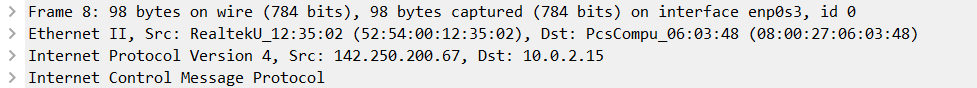
\includegraphics[width=\textwidth]{Imagens/13.png}
        \caption{Captura de um pacote ICMP}
        \vspace{-10pt}
    \end{figure}
    
    Na nossa opinião, a forma mais correta de calcular o \textit{overhead,} resultante da utilização de um determinado protocolo de transporte, respeita a seguinte fórmula:

    \vspace{-10pt}
        
    \[
      \text{\textit{overhead}} 
      = \dfrac
        {\sum_{i=1}^{n} h_i}
        {\sum_{i=1}^{n} p_i + h_i}
        \times 100
    \]
    \vspace{-10pt}
    \[\text{\textit{n = number of packets}}\]
    \vspace{-22pt}
    \[\text{\textit{h = transport protocol header size}}\]
    \vspace{-22pt}
    \[\text{\textit{p = transport protocol playload size}}\]

    
    Infelizmente não encontramos nenhuma opção no \textit{Wireshark} capaz de fornecer um pequeno resumo que contivesse os tamanhos individuais dos diversos segmentos capturados, todavia foi possível obter uma média desses tamanhos que permite realizar o cálculo do \textit{overhead.}

    \newpage
    \begin{figure}[hb!]
        \centering
        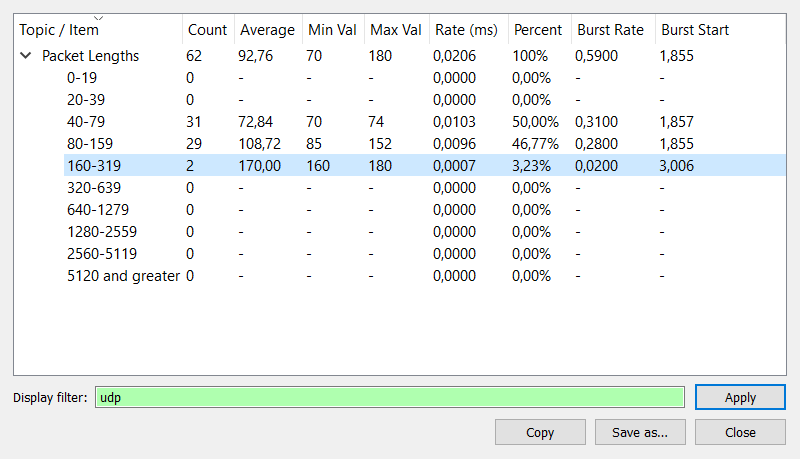
\includegraphics[width=0.6\textwidth]{Imagens/12.png}
        \caption{Sumário do tamanho dos segmentos}
        \vspace{-10pt}
    \end{figure}

    Após termos obtido este sumário ficámos bastante satisfeitos, contudo mais tarde percebemos que não o podíamos utilizar, pois os tamanhos apresentados não eram referentes ao \textit{playload} do protocolo de transporte, mas sim dos pacotes num todo, consequentemente acabámos por efetuar o cálculo do \textit{overhead} ao selecionar alguns pacotes aleatórios.
    
    \vspace{5pt}
    \textbf{\large Traceroute}
    \vspace{-15pt}

    \[
      \text{\textit{overhead}} 
      = \dfrac
        {8 \times 40}
        {32 \times 22 + 44 + 52 \times 8 + 56 \times 9 + 8 \times 40}
        \times 100
    \simeq 16.09
    \]

    \textbf{\large FTP}
    \vspace{-15pt}

    \[
      \text{\textit{overhead}} 
      = \dfrac
        {320}
        {839}
        \times 100
    \simeq 38.14
    \]

    \textbf{\large TFTP}
    \vspace{-15pt}

    \[
      \text{\textit{overhead}} 
      = \dfrac
        {96}
        {2872}
        \times 100
    \simeq 3.34
    \]

    \textbf{\large ssh}
    \vspace{-15pt}

    \[
      \text{\textit{overhead}} 
      = \dfrac
        {544}
        {4850}
        \times 100
    \simeq 11.22
    \]

    \textbf{\large telnet}
    \vspace{-15pt}

    \[
      \text{\textit{overhead}} 
      = \dfrac
        {140}
        {679}
        \times 100
    \simeq 20.62
    \]

    \textbf{\large browser}
    \vspace{-15pt}

    \[
      \text{\textit{overhead}} 
      = \dfrac
        {240}
        {9665}
        \times 100
    \simeq 2.48
    \]

    \textbf{\large nslookup}
    \vspace{-15pt}

    \[
      \text{\textit{overhead}} 
      = \dfrac
        {48}
        {378}
        \times 100
    \simeq 12.69
    \]

    \textbf{\large BitTorrent}
    \vspace{-15pt}

    \[
      \text{\textit{overhead}} 
      = \dfrac
        {212}
        {1352}
        \times 100
    \simeq 15.68
    \]

    \textbf{\large XMPP}
    \vspace{-15pt}

    \[
      \text{\textit{overhead}} 
      = \dfrac
        {422}
        {1996}
        \times 100
    \simeq 21.14
    \]

    \textbf{\large Git}
    \vspace{-15pt}

    \[
      \text{\textit{overhead}} 
      = \dfrac
        {526}
        {2135}
        \times 100
    \simeq 24.63
    \]
    

    
    \vspace{5pt}
    Ao comparar os \textit{overheads} associados aos vários protocolos da camada de transporte, percebemos claramente que o FTP apresenta um valor muito superior aos restantes, contudo, uma vez que o cálculo baseou-se somente num conjunto de segmentos escolhidos aleatoriamente por nós, é muito provável que tal valor não corresponda à realidade.